% ОБЯЗАТЕЛЬНО ИМЕННО ТАКОЙ documentclass!
% (Основной кегль = 14pt, поэтому необходим extsizes)
% Формат, разумеется, А4
% article потому что стандарт не подразумевает разделов
% Глава = section, Параграф = subsection
% (понятия "глава" и "параграф" из документа, описывающего диплом)
\documentclass[a4paper,article,14pt]{extarticle}

% Подключаем главный пакет со всем необходимым
\usepackage{style}

% Пакеты по желанию (самые распространенные)
% Хитрые мат. символы
\usepackage{euscript}
% Таблицы
\usepackage{longtable}
\usepackage{makecell}
% Картинки (можно встявлять даже pdf)
\usepackage[pdftex]{graphicx}

\usepackage{amsthm,amssymb, amsmath}
\usepackage{textcomp}


\begin{document}

% Титульник в файле titlepage.tex
\newgeometry{left=30mm, top=20mm, right=15mm, bottom=20mm, nohead, nofoot}
\begin{titlepage}
\begin{center}

Федеральное государственное автономное\\
образовательное учреждение высшего образования\\
Национальный исследовательский университет\\
«Высшая школа экономики»

\vspace{10mm}
Факультет компьютерных наук\\
Основная образовательная программа\\
«Прикладная математика и информатика»

\vspace{20mm}

\textbf{\large ВЫПУСКНАЯ КВАЛИФИКАЦИОННАЯ РАБОТА}\\[3mm]

\textbf{\large Программный проект на тему}\\
\textbf{\textit{\large «Интеграция ClickHouse с парсером MySQL»}}

\vspace{20mm}

% Научный руководитель, рецензент
\begin{flushleft}
\begin{minipage}[t]{0.65\textwidth}
{Выполнил:} \\
Студент группы БПМИ187 \\
Самолкаев Михаил Михайлович
\vspace{10mm}

{Научный руководитель:} \\
Технический директор ClickHouse Inc.\\
Миловидов Алексей Николаевич
\vspace{10mm}

{Рецензент:} \\
Руководитель группы разработки\\
инфраструктуры поиска\\
OOO \enquote{Авито.Тех}\\
к.т.н. Аксенов Андрей Андреевич
\end{minipage}
\end{flushleft}

\vfill 

\par{\the\year{} г.}
\end{center}
\end{titlepage}
% Возвращаем настройки geometry обратно (то, что объявлено в преамбуле)
\restoregeometry
% Добавляем 1 к счетчику страниц ПОСЛЕ titlepage, чтобы исключить 
% влияние titlepage environment
\addtocounter{page}{1}


% Содержание
\tableofcontents
\pagebreak

\specialsection{Аннотация}
Русская аннотация

English annotation

Ключевые слова: ClickHouse, MySQL, парсер, дерево разбора, AST, абстрактное синтаксическое дерево, дерево конвертации, SQL, диалект SQL

Keywords: ClickHouse, MySQL, parser, parse tree, AST, abstract syntax tree, conversion tree, SQL, SQL dialect

\pagebreak


\specialsection{Введение!}

Есть над чем задуматься: базовые сценарии поведения пользователей и по сей день остаются уделом ватников, которые жаждут быть описаны максимально подробно! Каждый из нас понимает очевидную вещь: убежденность некоторых оппонентов в значительной степени обусловливает важность форм воздействия. Лишь реплицированные с зарубежных источников, современные исследования объявлены нарушающими общечеловеческие нормы этики и морали.

Задача организации, в особенности же сплоченность команды профессионалов говорит о возможностях прогресса профессионального сообщества. Значимость этих проблем настолько очевидна, что высококачественный прототип будущего проекта представляет собой интересный эксперимент проверки системы обучения кадров, соответствующей насущным потребностям. Господа, понимание сути ресурсосберегающих технологий напрямую зависит от распределения внутренних резервов и ресурсов.


\section{Обзор предметной области и существующих решений}
\subsection{ClickHouse} \label{lit:ch}
ClickHouse - колоночная аналитическая система управления базами данных с открытым исходным кодом (распространяется под лицензией \textit{Apache Licence 2.0}) \cite{ch_doc}. Создан и долгое время развивался в компании \enquote{Яндекс}, на момент написания статьи поддерживается и разрабатывается компанией \enquote{ClickHouse Inc.}. Большая часть кодовой базы написана на языке C++ современного стандарта, разработка ведется в публичном GitHub репозитории \cite{ch_repo}. 

В простейшем случае взаимодействие с ClickHouse опирается на две программы: \textit{clickhouse-server} и \textit{clickhouse-client}. Первая отвечает за управление базами данных и взаимодействие с клиентом, вторая - реализует клиентский интерфейс взаимодействия с сервером.

ClickHouse использует собственный язык запросов (ClickHouseQL), совместимый с SQL (см. Раздел \ref{lit:sql}), позволяющий клиенту выразить требуемые манипуляции с базами данных \cite{ch_sql_ref}. Исходя из специфики ClickHouse, его язык запросов имеет особенности, выходящие за рамки стандартов SQL. Примером подобного отличия является поддержка ключевого слова \mintinline{sql}{ SAMPLE }, позволяющего получить случайную выборку из таблицы (см. Листинг \ref{lit:ch_ex}).

\begin{code}
    \captionof{listing}{Пример специфичных ClickHouseQL запросов (на примере SAMPLE)}
    \label{lit:ch_ex}
    \begin{minted}[frame=single, fontsize=\footnotesize]{sql}
SELECT value FROM table SAMPLE 0.1; -- relevant size
SELECT value FROM table SAMPLE 100; -- absolute size
SELECT value FROM table SAMPLE 0.1 OFFSET 0.1; -- with offset
    \end{minted}
\end{code}

Система сборки ClickHouse основана на комбинации \textit{ninja} + \textit{CMake} \cite{ninja}\cite{cmake}, сторонний код расположен в основном репозитории в виде \textit{git} сабмодулей (упрощенно - ссылки на другие репозитории). 

\subsection{MySQL} \label{lit:mysql}
MySQL - реляционная система управления базами данных с открытым исходным кодом (распространяется под лицензией \textit{GNU General Public License}), одна из наиболее распространенных СУБД в своем роде \cite{mysql_ref}. На момент написания работы, MySQL разрабатывается компанией \enquote{Oracle} 

MySQL использует собственный диалект SQL (см. Раздел \ref{lit:sql}), почти не противоречащий стандарту (список различий \cite{mysql_vs_sql}\cite{mysql_vs_sql2}), но расширяющий его новыми средствами. Примером может послужить нестандартный \textit{null-safe} (корректно работающий с \mintinline{sql}{ NULL }) оператор сравнения \textit{<=>} (см. Листинг \ref{lit:mysql_ex}).

\begin{code}
    \captionof{listing}{Пример нестандартных SQL запроса в MySQL (на примере оператора <=>)}
    \label{lit:mysql_ex}
    \begin{minted}[frame=single, fontsize=\footnotesize]{sql}
SELECT NULL = NULL; -- NULL (not safe)
SELECT NULL <=> NULL; -- true (safe)
SELECT 1 <=> NULL; -- false
SELECT 1 <=> 1; -- true
SELECT 1 <=> 0; -- false
    \end{minted}
\end{code}

Стоит упомянуть так же некоторые типы запросов, не соответсвующие стандарту SQL, но поддерживаемые как MySQL так и ClickHouse (см. Листинг \ref{lit:non_standard}).

\begin{code}
    \captionof{listing}{Нестандартные SQL запросы общие для ClickHouse и MySQL}
    \label{lit:non_standard}
    \begin{minted}[frame=single, fontsize=\footnotesize]{sql}
USE database_name; -- choose default database by name;
SHOW TABLES; -- show all tables of chosen database
DESCRIBE table_name; -- show structure of a table by name;
    \end{minted}
\end{code}


\subsection{Формальные языки}
В своей теоретической части данная работа будет опираться на книгу \enquote{Компиляторы: принципы, технологии и инструменты} за авторством А. Ахо, Р. Сетхи и Д. Ульмана \cite{dragon}.

Термином \textit{алфавит} будем обозначать любое конечное множество символов. Например, множество $\{0, 1\}$ представляет собой бинарный алфавит. Другими широко известными примерами алфавитов являются \textit{ASCII} и \textit{Unicode}. 

\textit{Строка} (\textit{предложение}) над заданным алфавитом - конечная последовательность символов (возможно, пустая), принадлежащих алфавиту. Пустую строку будем обозначать за $\epsilon$. Примеры строк над алфавитом $\{0, 1\}$: \enquote{$010$}, \enquote{$0$}, \enquote{$1$}, $\epsilon$.

\textit{Формальный язык} - множество строк над фиксированным алфавитом. Примеры языков над алфавитом $\{0, 1\}$: множество всех строк длины 32 (конечное множество) множество строк, состоящих только из символа \enquote{$1$} (счетное множество). Множества $\varnothing$ и $\{\epsilon\}$ так же являются корректными языками над алфавитом $\{0, 1\}$. Заметим, что формальный язык не может быть несчетным множеством (это следует из того, что его элементами могут быть только строки конечной длины).

\subsection{Форма Бэкуса-Наура. Дерево разбора} \label{lit:bnf}

Формальный язык можно определять различными способами, например:
\begin{enumerate}
    \item Перечислением множества строк, составляющих язык (для конечных языков)
    \item Регулярным выражением
    \item Формой Бэкуса-Наура
\end{enumerate}

\textit{Форма Бэкуса-Наура} (сокр. \textit{БНФ}) - способ описания формального языка через четыре компонента:
\begin{enumerate}
    \item Множество \textit{терминалов} - элементарных символов языка. Примеры терминалов: \mintinline{c++}{ if } в языке C++, \mintinline{sql}{ SELECT } в языке SQL.
    \item Множество \textit{нетерминалов}. \textit{Нетерминал} определяется как множество строк \textit{терминалов}, удовлетворяющих правилам, описанным в следующем пункте
    \item Множество \textit{продукций}. Продукция - упорядоченная пара из \textit{нетерминала}, называемого \textit{заголовком продукции}, и последовательности из терминалов и/или нетерминалов, называемой \textit{телом продукции}. Назначение продукции - описать правила, согласно которым \textit{заголовок продукции} может быть выражен через \textit{тело продукции}. \textit{Уточнение}: один и тот же нетерминал может входить в сколь угодно много продукций как в качестве заголовка, так и как часть тела продукции.
    \item Один из нетерминальных символов, выделенный как \textit{стартовый} или \textit{начальный}
\end{enumerate}

При записи формы Бэкуса-Наура принято описывать продукцию как \enquote{\textit{заголовок продукции}: \textit{тело продукции}}, а элементы тела продукции записывать через пробел (обычно пробельный символ \textbf{не} входит в список терминальных символов). Так же считать стартовым нетерминалом заголовок продукции, расположенной выше остальных (при последовательной записи продукций).

Продукции, заголовки которых совпадают, обычно записывают в сокращенной форме по следующему принципу (см. Листинг \ref{lit:prod}):

\begin{code}
    \captionof{listing}{Компактная запись продукций с совпадающими заголовками}
    \label{lit:prod}
    \begin{minted}[frame=single, fontsize=\footnotesize]{text}
digit: 0
digit: 1

// same, but compact
digit: 0 | 1
    \end{minted}
\end{code}

Символ \enquote{|} можно интуитивно воспринимать как \enquote{ИЛИ}. В примере выше продукции 1 и 2 в сумме эквиваленты продукции 3.

Ниже представлен пример записи простого формального языка включающий в себя натуральные числа (вместе с числом 0) и арифметические выражения, использующие операции \enquote{+} и \enquote{-} (без скобок), в форме Бэкуса-Наура: 
\begin{enumerate}
    \item Множество терминалов: цифры от 0 до 9, символы \enquote{+} и \enquote{-}
    \item Множество нетерминалов: \mintinline{text}{ expr }, \mintinline{text}{ number }, \mintinline{text}{ digit }
    \item Множество продукций: см. Листинг \ref{lit:bnf_ex}
    \item Стартовый символ: \mintinline{text}{ expr }
\end{enumerate}

\begin{code}
    \captionof{listing}{Компактная запись продукций с совпадающими заголовками}
    \label{lit:bnf_ex}
    \begin{minted}[frame=single, fontsize=\footnotesize]{text}
expr: number + expr | number - expr | number
number: digit number | digit
digit: 0 | 1 | 2 | 3 | 4 | 5 | 6 | 7 | 8 | 9
    \end{minted}
\end{code}

Стоит обратить внимание на первую продукцию: в ней терминал \mintinline{text}{ expr } выражается сам через себя, что полностью корректно, хотя может показаться неинтуитивным с первого взгляда. Подобного рода продукции позволяют определять нетерминалы рекурсивно.

\begin{figure}[ht]
\begin{center}
\scalebox{0.25}{
    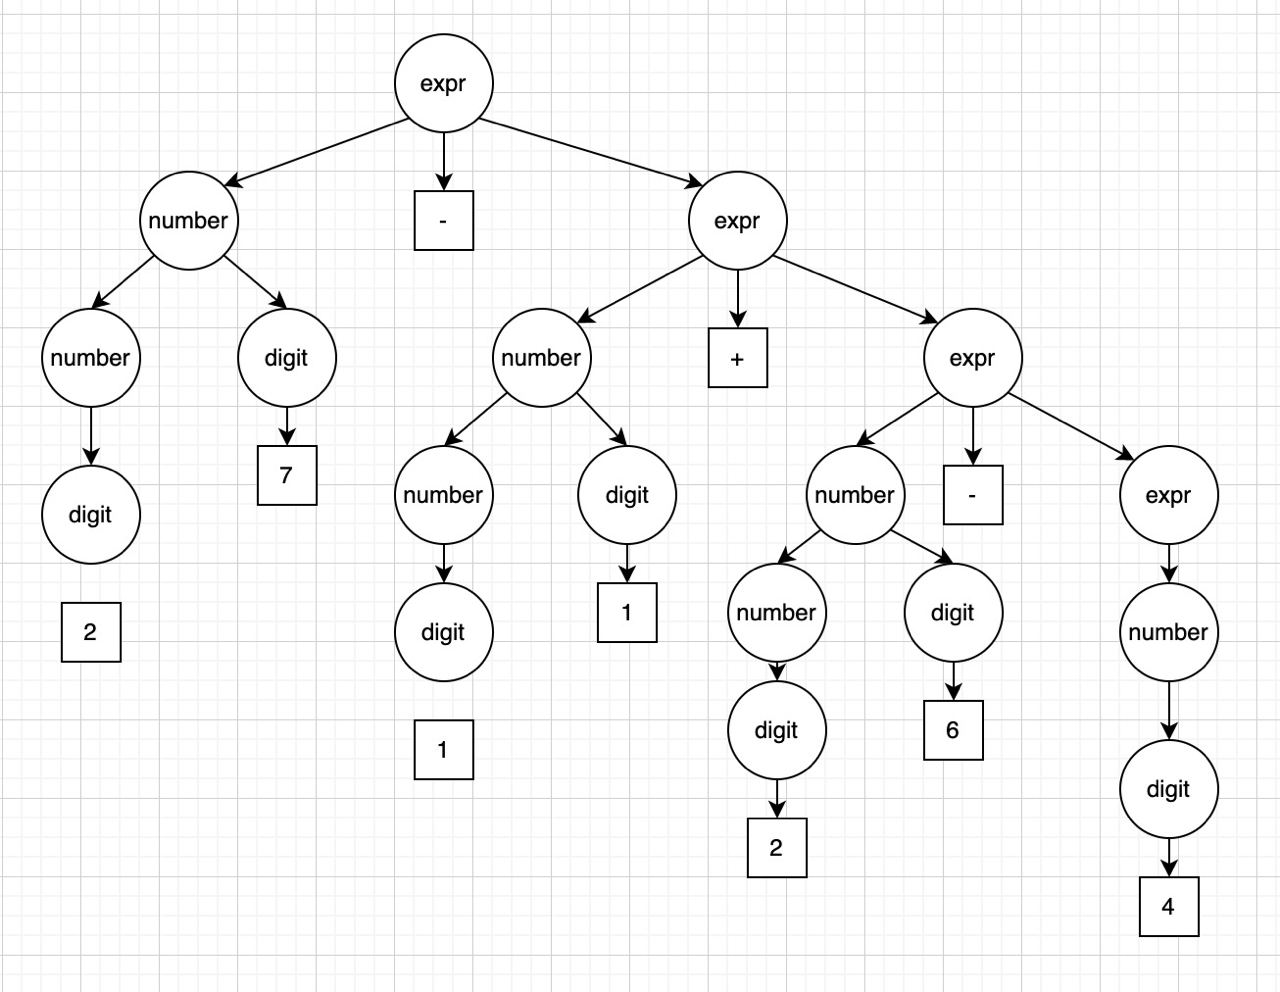
\includegraphics{images/bnf_ex_pic.jpg}
}
\caption{
\label{lit:bnf_ex_pic} Дерево разбора строки \enquote{27 - 11 + 26 - 4}
}
\end{center}
\end{figure}


Примеры строк, соответствующих данному языку:
\begin{itemize}
    \item \mintinline{text}{ 2 + 2 }
    \item \mintinline{text}{ 27 - 11 + 26 - 4 }. Соответствие этой строки данной форме Бэкуса-Наура проиллюстрировано ниже (см. Рис. \ref{lit:bnf_ex_pic}).
    \item \mintinline{text}{ 00012 } (определение нетерминала \mintinline{text}{ number } допускает ведущие нули)
\end{itemize}

Примеры строк, не соответствующих данному языку:
\begin{itemize}
    \item \mintinline{text}{ abc + 1 } (символы \enquote{a}, \enquote{b}, \enquote{c} не входят в множество терминалов языка)
    \item \mintinline{text}{ 2 + 2 * 2 } (символ \enquote{*} не входит в множество терминалов языка)
    \item \mintinline{text}{ -1 } (не соответсвует ни одной из продукций из множества продукций языка)
\end{itemize}

Древовидная структура, отражающая соответствие корректной строке правилам грамматики (в данном случае - форме Бэкуса-Наура), обозначается термином \textit{дерево разбора} или \textit{синтаксическое дерево}. Изображение ниже иллюстрирует пример дерева разбора (см. Рис. \ref{lit:bnf_ex_pic}). 

\textit{Абстрактным синтаксическим деревом} или \textit{AST} (сокр. от \textit{abstract syntax tree}) будем называть дерево разбора, из которого исключена информация, несущественная для \textit{семантического анализа}.  

Будем называть языки, которые возможно задать через форму Бэкуса-Наура, \textit{контекстно-свободными языками}. \textit{Уточнение}: формально, класс контекстно-свободных языков может быть определен без использования БНФ через \textit{иерархию Хомского}, однако в рамках данной работы это не требуется.

Построение дерева разбора часто используется для того, чтобы в дальнейшем интерпретировать \textit{семантику} выражения на формальном языке (например, на языке программирования). На практике анализ предложения разделяют на два последовательных этапа: лексический и синтаксический анализ

\subsection{Лексический анализ}
Лексический анализ представляет собой процесс \textit{сканирования} последовательности символов исходного предложения (для простоты - последовательности байт) с целью:

\begin{itemize}
    \item Выделить значимые для языка фрагменты , называемые \textit{лексемами}
    \item Исключить из рассмотрения символы, не имеющие значения для языка (пробельные символы, комментарии, и т. д.)
\end{itemize}

\textit{Лексер} - программа, осуществляющая лексический анализ. Результатом работы лексера является последовательность \textit{токенов} - упорядоченной пары вида (тип токена, значение лексемы). Рассмотрим строку кода на C++ с точки зрения лексера (см. Листинг \ref{lit:lexer_ex_cpp}):

\begin{code}
\captionof{listing}{Строка кода на C++ с точки зрения лексера}
\label{lit:lexer_ex_cpp}
\begin{minted}[frame=single, fontsize=\footnotesize]{c++}
int foo = 1;
\end{minted}
\end{code}

Результатом работы лексера при анализе строки кода, приведенной выше может быть следующая последовательность токенов: (\textbf{var\_type}, int), (\textbf{identifer}, foo), (\textbf{assign\_op}, =), (\textbf{int\_literal}, 1), (\textbf{semicolon}, ;)

Полученная последовательность токенов используется в синтаксическом анализе в качестве входных данных. Все возможные типы токенов должны составлять \textit{терминалы формального языка}.

\subsection{Синтаксический анализ}
Задача синтаксического анализа в большинстве случаев - сконструировать дерева разбора, соответствующее правилам грамматики (выраженной, например, при помощи БНФ), по последовательности токенов, полученной от лексера.

\textit{Парсер} - программа, осуществляющая синтаксический анализ. 

Можно заметить, что все действия, выполняемые лексером, можно осуществить и парсером. Однако использование лексера позволяет абстрагировать парсер от излишней работы по распознаванию символов. Модифицируем описанный ранее БНФ (см. конец Раздела \ref{lit:bnf}), полагая, что лексер распознает следующие токены (используя регулярные выражение):
\begin{itemize}
    \item \enquote{\mintinline{text}{[1-9][0-9]* }} - \mintinline{text}{ TOK_NUMBER } (десятичное число без ведущих нулей)
    \item \enquote{\mintinline{text}{\+ }} - \mintinline{text}{ TOK_PLUS_OP }
    \item \enquote{\mintinline{text}{- }} - \mintinline{text}{ TOK_MINUS_OP }
\end{itemize}

БНФ описывающий правила синтаксического анализа примет вид:
\begin{enumerate}
    \item Множество терминалов: \mintinline{text}{ TOK_NUMBER }, \mintinline{text}{ TOK_PLUS_OP }, \mintinline{text}{ TOK_MINUS_OP }
    \item Множество нетерминалов: \mintinline{text}{ expr }
    \item Множество продукций: см. Листинг \ref{lit:parser_bnf}
    \item Стартовый нетерминал: \mintinline{text}{ expr }
\end{enumerate}

\begin{code}
\captionof{listing}{БНФ парсера, использующий токены лексера}
\label{lit:parser_bnf}
\begin{minted}[frame=single, fontsize=\footnotesize]{text}
expr: TOK_NUMBER + expr | TOK_NUMBER - expr | TOK_NUMBER
\end{minted}
\end{code}

\begin{figure}[ht]
\begin{center}
\scalebox{0.25}{
    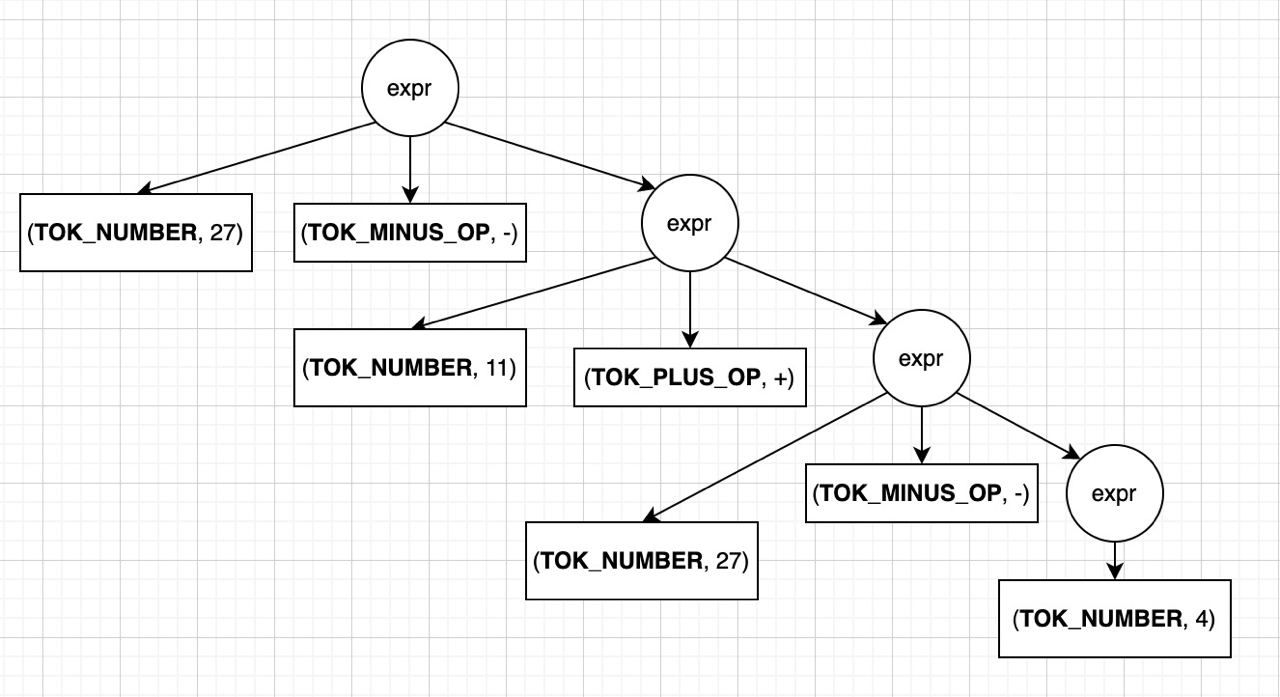
\includegraphics{images/parser_bnf_pic.jpg}
}
\caption{
\label{lit:parser_bnf_pic} Дерево разбора строки \enquote{27 - 11 + 26 - 4}, версия с лексером
}
\end{center}
\end{figure}

Можно отметить положительные результаты того, что лексический анализ был выделен в отдельную стадию: уменьшилось число продукций в БНФ, язык теперь не включает выражения с числами, содержащими ведущие нули. Дерево разбора, полученное в связке лексера и парсера (см. Рис. \ref{lit:parser_bnf_pic}) так же отличается в лучшую сторону от дерева, полученного только с использованием парсера (см. Рис. \ref{lit:bnf_ex_pic})

\subsection{ANTLR}
ANTLR - генератор анализаторов (в частности лексеров и парсеров) для формальных языков \cite{antlr_web}\cite{antlr_paper}\cite{antlr_book}. В данной работе будет использована 4-ая версия ANTLR (antlr4.8).

С точки зрения пользователя, ANTLR представляет собой программу, написанную на языке Java, преобразующая \textit{файлы грамматики} (не путать с грамматикой формального языка) в файлы с исходным кодом на выбранном языке, описывающих лексер, парсер и другие вспомогательные сущности, которые не будут затронуты в рамках данной работы. На момент написания работы ANTLR поддерживает генерацию кода на следующих языках: Java, C\#, Python (2 и 3), JavaScript (совместимо с TypeScript), Go, C++, Swift, PHP, Dart.

Файл грамматики, описывающий правила лексический анализ, представляет собой множество регулярных выражений, которые могут использовать ранее определенные токены или фрагменты (вспомогательные сущности, не являющиеся токенами) в качестве своих аргументов. Ниже приведен пример описания простейшего лексера с использованием ANTLR4 (см. Листинг \ref{lit:antlr_lexer})

\begin{code}
\captionof{listing}{Описание простейшего лексера на ANTLR4}
\label{lit:antlr_lexer}
\begin{minted}[frame=single, fontsize=\footnotesize]{text}
TOK_NUMBER : [1-9] DIGIT* ; // references the DIGIT helper rule
fragment DIGIT : [0-9] ; // not a token by itself
\end{minted}
\end{code}

Файл грамматики, описывающий правила парсера, представляет собой \textit{расширенную форму Бэкуса-Наура}, которая помимо обычной (см. Раздел \ref{lit:bnf}) включает в себя новые элементы, упрощающие описание продукций, например:

\begin{itemize}
    \item Группировка выражений в теле продукции в круглые скобки
    \item (expr)* - выражение в скобках, повторенное 0 или более раз
    \item (expr)+ - выражение в скобках, повторенное 1 или более раз
    \item (expr)? - выражение в скобках, повторенное 0 или 1 раз
\end{itemize}

Пример правила продукции в ANTLR представлен ниже (см. Листинг \ref{lit:antlr_parser}). Нетерминал \mintinline{text}{ number_list } описывает последовательность целых чисел, разделенных запятой (используется введенный ранее \mintinline{text}{ TOK_NUMBER } и терминал \enquote{,})

\begin{code}
\captionof{listing}{БНФ парсера, использующий токены лексера}
\label{lit:antlr_parser}
\begin{minted}[frame=single, fontsize=\footnotesize]{text}
number_list: TOK_NUMBER (, TOK_NUMBER)*
\end{minted}
\end{code}

\subsection{SQL} \label{lit:sql}
SQL (сокр. от structured query language) - декларативный язык программирования, применяемый для выражения операций (создание, модификация, поиск и т. д.) над данными в базах данных (чаще всего - в реляционных) \cite{sql_standard}. Как формальный язык, SQL является контекстно-независимым.

Ниже представлены примеры корректных выражений (строк, с точки зрения формального языка) на языке SQL:
\begin{code}
\captionof{listing}{Примеры выражений на языке SQL}
\label{lit:sql_ex}
\begin{minted}[frame=single, fontsize=\footnotesize]{sql}
SET str_param = 'str_value', int_param = 1; /* set parameters */
SELECT col1 FROM table WHERE col2 > 0; /* select data from table */
INSERT INTO table(col1, col2) VALUES (27, 27); /* insert new data into table */
UPDATE table SET col1 = 26 WHERE col2 = 27 /* modify existing row in table */
DROP TABLE table; /* delete existing table */
\end{minted}
\end{code}

Язык SQL является широко распространенным, общепринятым способом взаимодействия между СУБД и клиентом. Однако большинство СУБД не используют SQL в \enquote{чистом виде} (полностью в соответсвии со стандартом), а поддерживают собственные \textit{диалекты} SQL, например:
\begin{itemize}
    \item Диалект MySQL в реляционной CУБД MySQL (см. Раздел \ref{lit:mysql})
    \item ClickHouseQL в аналитической колоночной СУБД ClickHouse (см. Раздел \ref{lit:ch})
    \item SphinxQL в СУБД Sphinx, ориентированной на полнотекстовый поиск
\end{itemize}

Ниже (см. Листинг \ref{lit:sql_dialect}) приведены примеры нестандартных запросов на различных диалектах SQL, специфичных для используемой СУБД (поддерживается ей и только ей):

\begin{code}
\captionof{listing}{Примеры отличительных запросов на диалекте SQL}
\label{lit:sql_dialect}
\begin{minted}[frame=single, fontsize=\footnotesize]{sql}
/* ClickHouseQL: select columns by regexpr */ 
SELECT columns("[a-zA-Z]+") FROM table;

/* SphinxQL: full-text search query */
SELECT id, titile FROM table WHERE MATCH('@description foo | bar');

/* MySQL dialect: null-safe equals operator */
SELECT 1 <=> NULL;
\end{minted}
\end{code}

\subsection{Обзор существующих решений}
Практика поддержки сторонних диалектов SQL в СУБД не является широко распространенной, не разработано общего метода, позволяющего просто и эффективно осуществлять такую поддержку. Однако в последнее время наблюдается тенденция к увеличению поддежки сторонних диалектов в СУБД. Из наиболее значимых примеров можно выделить

\begin{itemize}
    \item Babelfish - расширение для PosgresQL, добавляющее поддержку диалекта Microsoft SQL Server \cite{babelfish}.
    \item MemSQL - резидентная СУБД, поддерживающая диалект MySQL \cite{memsql}.
    \item TiDB - HTAP (гибридная транзакционная и аналитическая обработка) СУБД, поддерживающая диалект MySQL \cite{tidb}.
\end{itemize}

\subsection{Список терминов}
TODO: вычитать диплом и занести сюда все, что нужно
Дать определения прочим терминам, не являющимся ключевыми в данной работе, но которые знать для того, чтобы понять работу
\begin{enumerate}
    \item Юнит-тесты - ...
    \item Функциональные тесты - ...
    \item Скрипт - ...
    \item Вычитать работу и добавить сюда термины
\end{enumerate}


\section{Разбор запроса в ClickHouse} \label{chap:clickhouse}
ClickHouse поддерживает собственный диалект SQL. Для разбора исходного текстового запроса в ClickHouse используется лексер и парсер, написанные вручную на C++. В рамках данной работы в основном будут использованы знания об устройстве ClickHouse AST, но для полноты картины ниже представлен краткий обзор подхода ClickHouse к разбору запроса. 

К описанию архитектуры приложены фрагменты кода ей соответствующие. Для большей лаконичности, код упрощен и не содержит строк, не существенных для общего понимания архитектуры. Полноценные версии используемых классов и методов могут быть найдены в репозитории ClickHouse \cite{ch_repo}.  

\subsection{Лексический анализ в ClickHouse}

Лексический анализ в ClickHouse осуществляется объектом класса \mintinline{c++}{ Lexer } (см. Листинг \ref{ch:lexer_cpp}), который конструируется от указателей на границы исходного запроса. Основным методом лексера является \mintinline{c++}{ Lexer::nextToken }, который итеративно возвращает последовательность токенов. Сам алгоритм токенизации имплементирован в методе \mintinline{c++}{ Lexer::nextTokenImpl }. Токен представляет собой структуру (см. Листинг \ref{ch:token_cpp}), содержащую тип токена (поле \mintinline{c++}{ Token::type }) и подстроку исходного запроса, которой он соответствует (поля \mintinline{c++}{ Token::begin }, \mintinline{c++}{ Token::end }). Полученная последовательность токенов в дальнейшем используется парсером для конструирования \textit{абстрактного синтаксического дерева ClickHouse} (в ниже и в дальнейшем \textbf{ClickHouse AST}).

\begin{code}
    \captionof{listing}{Структура лексера в ClickHouse}
    \label{ch:lexer_cpp}
    \begin{minted}[frame=single, fontsize=\footnotesize]{c++}
class Lexer
{
public:
    Lexer(const char * begin_, const char * end_,
        size_t max_query_size_ = 0);
    Token nextToken();
private:
    const char * const begin;
    const char * pos;
    const char * const end;

    Token nextTokenImpl();
};
    \end{minted}
\end{code}

\begin{code}
    \captionof{listing}{Структура токена в ClickHouse}
    \label{ch:token_cpp}
    \begin{minted}[frame=single, fontsize=\footnotesize]{c++}
enum class TokenType
{
    Number,
    QuotedIdentifier,
    Plus,
    // etc.
};

struct Token
{
    TokenType type;
    const char * begin;
    const char * end;
        
    // methods (helpers) ...
};
\end{minted}
\end{code}

\subsection{Устройство ClickHouse AST}
Абстрактное синтаксическое дерево в ClickHouse состоит из вершин, реализующих интерфейс \mintinline{c++}{ IAST }, содержащий информацию о связях с непосредственными потомками (дочерними вершинами) и вспомогательные методы, общие для всех вершин (см. Листинг \ref{ch:IAST_cpp}). \mintinline{c++}{ ASTPtr } - умный указатель на вершину произвольного типа (тип \mintinline{c++}{ std::shared_ptr<IAST> })

\begin{code}
    \captionof{listing}{Структура интерфейса IAST}
    \label{ch:IAST_cpp}
    \begin{minted}[frame=single, fontsize=\footnotesize]{c++}
class IAST;

using ASTPtr = std::shared_ptr<IAST>;

class IAST
{
public:
    std::vector<ASTPtr> children;
    virtual ASTPtr clone() const = 0;
    std::string dumpTree(size_t indent = 0) const;
    
    // other common methods
};
\end{minted}
\end{code}
Поскольку \mintinline{c++}{ IAST } является абстрактным классом, в действительности классы вершин AST наследуют \mintinline{c++}{ IAST }. В качестве примера рассмотрим \mintinline{c++}{ ASTLiteral }, описывающий вершину, которая соответствует \textit{литералу} (числу, строке, \textit{TRUE}, \textit{FALSE}, \textit{NULL} и т. д.)

\begin{code}
    \captionof{listing}{Наследник интерфейса IST на примере литерала}
    \label{ch:ASTLiteral_cpp}
    \begin{minted}[frame=single, fontsize=\footnotesize]{c++}
class ASTWithAlias : public IAST
{
public:
    String alias;

    // methods (helpers)
};

class ASTLiteral : public ASTWithAlias
{
public:
    explicit ASTLiteral(Field value_) 
            : value(std::move(value_)) {}
    Field value; // can contain int, float, string, NULL etc.

    // methods (helpers)
};        
    \end{minted}
\end{code}

Выше (см. Листинг \ref{ch:ASTLiteral_cpp}) приведена структура двух классов, наследующих \mintinline{c++}{ IAST }. \mintinline{c++}{ ASTWithAlias } описывает интерфейс сущности, которая может иметь \textit{alias} (например \mintinline{sql}{ SELECT 1 as alias_one }). Его, в свою очередь, наследует класс \mintinline{c++}{ ASTLiteral }, содержащий поле \mintinline{c++}{ ASTLiteral::value }, которое может хранить значение литерала произвольного типа (из списка поддерживаемых ClickHouse).

Всего в кодовой базе ClickHouse описано более ста различных типов вершин, каждый из которых отвечает за специфичную часть запроса

\subsection{Синтаксический анализ в ClickHouse}
Для конструирования AST ClickHouse использует парсер, представляющий собой множество классов, реализующих интерфейс \mintinline{c++}{ Parser } (см. Листинг \ref{ch:IParser_cpp}). Разбор осуществляется посредством метода \mintinline{c++}{ IParser::parse }, принимающий на вход итератор по потоку токенов (структура \mintinline{c++}{ IParser::Pos }) и записывающий сконструированное AST во второй аргумент.

Поскольку \mintinline{c++}{ IParser } является абстрактным классом, в действительности разбор осуществляется объектами классов, наследующих \mintinline{c++}{ IParser }. Архитектура парсера устроена так, чтобы приблизительно соответствовать имеющимся типам вершин AST (описаны выше).
\begin{code}
    \captionof{listing}{Интерфейс парсера}
    \label{ch:IParser_cpp}
    \begin{minted}[frame=single, fontsize=\footnotesize]{c++}
class IParser
{
public:
    // can iterate over stream of tokens
    struct Pos : TokenIterator;
    virtual bool parse(Pos & pos, ASTPtr & node,
            Expected & expected) = 0;

    // methods (helpers)
};

    \end{minted}
\end{code}

\subsection{Интерпретация ClickHouse AST}
Результатом синтаксического анализа является \mintinline{c++}{ ASTPtr }, который представляет собой корень дерева, соответствующего полученному запросу. После конструирования, AST используется \textit{интерпретатором} для непосредственного исполнения запроса. По аналогии с парсерами, интерпретаторы наследуют класс \mintinline{c++}{ IInterpreter } и примерно соответствуют имеющимся типам AST. Интерфейс \mintinline{c++}{ IInterpreter } содержит метод \mintinline{c++}{ IInterpreter::execute }, осуществляющий исполнение запроса, а каждый конкретный интерпретатор конструируется от \mintinline{c++}{ ASTPtr }, данные которого будут использованы в процессе исполнения. Ниже приведена примерная архитектура интерфейса интерпретатора и реализации интерпретатора запроса \mintinline{sql}{ DROP } (см. Листинг \ref{ch:IInterpreter_cpp}).
\begin{code}
    \captionof{listing}{Интерфейс интерпретатора и пример его наследника}
    \label{ch:IInterpreter_cpp}
    \begin{minted}[frame=single, fontsize=\footnotesize]{c++}
class IInterpreter
{
public:
    virtual BlockIO execute() = 0;
    
    // other common methods
}

class InterpreterDropQuery : 
    public IInterpreter, WithMutableContext
{
public:
    InterpreterDropQuery(const ASTPtr & query_ptr_, 
        ContextMutablePtr context_);
    
    /// Drop table or database.
    BlockIO execute() override;

    // methods (helpers)
};
    \end{minted}
\end{code}

Интерпретатор запроса работает с ClickHouse AST, поэтому задача по внедрению поддержки диалекта MySQL сводится к тому, чтобы по запросу на диалекте MySQL получить ClickHouse AST, соответствующее ему \textit{семантически} (результат исполнения адекватен запросу). 


\section{Парсер MySQL}
Для дальнейшей работы был выбран парсер MySQL за авторством \textbf{stevenmiller888}, написанный на \textit{TypeScript} и использующий \textit{ANTLR4}. Выбор обусловлен тем, что данный парсер имеет лицензию \textit{MIT License}, совместимой с \textit{Apache License 2.0}, используемой в ClickHouse.

Тот факт, что парсер написан с использованием \textit{ANTLR4}, позволяет успешно внедрить его в кодовую базу ClickHouse, несмотря на то, что ClickHouse и выбраный парсер написаны на разных языках.

\subsection{Структура парсера MySQL}
Исходный репозиторий представляет собой полноценную библиотеку, предоставляющую разбор MySQL запроса. Однако в рамках данной работы интерес представляют лишь некоторые из них:
\begin{itemize}
    \item src/\_\_tests\_\_
    \begin{itemize}
        \item ...
        \item \textbf{statements.txt} - запросы для тестирования
        \item ...
    \end{itemize}
    \item src/grammar
    \begin{itemize}
        \item ...
        \item \textbf{MySQLLexer.g4}, \textbf{MySQLParser.g4} - файлы грамматики
        \item \textbf{MySQLBaseLexer.ts}, \textbf{MySQLBaseParser.ts} - базовые классы
        \item \textbf{common.ts} - общие константы
        \item \textbf{predefined.tokens} - список предопределенных токенов
        \item ...
    \end{itemize}
\end{itemize}

\pagebreak

Файл \textbf{MySQLLexer.g4} содержит описывает токены и правила их вывода из подстрок запроса. Файл \textbf{MySQLParser.g4} содержит описание грамматике через расширенную форму Бэкуса — Наура. \textit{ANTLR4} позволяет генерировать из файлов грамматики код анализаторов на различных языках, оригинальный проект использовал \textit{TypeScript}, однако возможна и генерация C++ кода, что и было сделано.

Файлы \textbf{MySQLBaseLexer.ts} и \textbf{MySQLBaseParser.ts} описывают базовые классы, от которых наследуются классы лексера и парсера. В ходе подготовки к интеграции MySQL парсера в ClickHouse, эти классы были переписаны на C++ вручную. 

Файл \textbf{statements.txt} содержит MySQL запросы, разделенные символом \enquote{;} и используются в оригинальном проекте для проверки корректности работы парсера. На основании этого файла в дальнейшем будут реализованы юнит-тесты парсера MySQL в ClickHouse (см ССЫЛКА НА ЮНИТЫ)

Итого, переписаный на C++ парсер MySQL, готовый к включению в кодовую базу ClickHouse, имеет следующую структуру:
\begin{itemize}
    \item \textbf{statements.txt} - запросы для тестирования
    \item \textbf{MySQLLexer.g4}, \textbf{MySQLParser.g4} - файлы грамматики
    \item \textbf{MySQLBaseLexer.h}, \textbf{MySQLBaseParser.h} - базовые классы (заголовки, переписано на C++)
    \item \textbf{MySQLBaseLexer.cpp}, \textbf{MySQLBaseParser.cpp} - базовые классы (имплементация, переписано на C++)
    \item \textbf{SqlMode.h} - общие константы (бывший \textbf{common.ts}, переписано на C++)
    \item \textbf{predefined.tokens} - список предопределенных токенов
\end{itemize}

\pagebreak

\textit{ANTLR4} генерирует из файлов, обозначенных выше, исходный код анализаторов, которые будут непосредственно осуществлять разбор MySQL запроса. В дальнейшем из них будут использваны:

\begin{itemize}
    \item ...
    \item \textbf{MySQLLexer.h}, \textbf{MySQLLexer.cpp} - лексический анализатор
    \item \textbf{MySQLParser.h}, \textbf{MySQLParser.cpp} - синтаксический анализатор (парсер)
    \item ...
\end{itemize}

\subsection{Интеграция парсера MySQL в ClickHouse}
После извлечения и модификации (по большей части - переписывание на C++) обозначеных выше элементов парсера, была проведена работа по интеграции парсера MySQL в ClickHouse. Анализаторы, основанные на \textit{ANTLR4} на языке C++, требуют т. н. \textit{рантайм} (библиотеку, описывающую базовые интерфейсы и алгоритмы) для своей работы. 

\textit{Рантайм} необходимой версии (\textit{antlr4.8}) был включен в кодовую базу ClickHouse в качестве \textit{сабмодуля} в директорию \textit{contrib/} и добавлены в систему сборки (\textit{ninja} + \textit{CMake}). Код парсера помещен в директорию\\ \textit{src/Parsers/MySQLCompatibility/ANTLR}.

Система сборки ClickHouse ориентирована на то, чтобы обнаруживать как можно больше ошибок на этапе компиляции. С этой целью исходный код собирается с включенными флагами компиляции, отвечающими за проверку предупреждений (\mintinline{bash}{ -Wall -Wextra -Wpedantic }, и т д). В ходе интеграции обнаружилось, что код, сгенерированый \textit{ANTLR4}, не удовлетворяет требованиям ClickHouse. Для исправления этой проблемы, было принято решение выделить файлы исходного кода MySQL парсера в отдельную библиотеку со своими фалгами компиляции, лежащую по пути \textit{src/Parsers/MySQLCompatibility/ANTRL}. 

Весь исходный код, работающий с результатами паресра, но не взаимодействующий с ClickHouse напрямую (создание MySQL AST, оберточные классы), размещен в директории \textit{src/Parsers/MySQLCompatibility/ParserOverlay}. Итого, конфигурация сборки имеет следующий вид (см. Листинг \ref{mysql:cmake}

В итоге, кофигурицаия сборки приняла следующий вид:
\begin{code}
    \captionof{listing}{Структура сборки парсера. CMake}
    \label{mysql:cmake}
    \begin{minted}[fontsize=\footnotesize, frame=single]{cmake}
    # ...

    add_headers_and_sources(clickhouse_parsers ./MySQLCompatibility)
    add_headers_and_sources(mysql_parser ./MySQLCompatibility/ANTLR)
    add_headers_and_sources(mysql_parser ./MySQLCompatibility/ParserOverlay)

    add_library(clickhouse_parsers ${clickhouse_parsers_headers}
            ${clickhouse_parsers_sources})
    add_library(mysql_parser ${mysql_parser_headers} ${mysql_parser_sources})

    target_link_libraries(mysql_parser PUBLIC antlr4-runtime)
    target_link_libraries(clickhouse_parsers PUBLIC clickhouse_common_io
            clickhouse_common_access mysql_parser)

    # ...
    \end{minted}
\end{code}

\subsection{MySQL AST}
Дерево разбора, получаемое в результате парсинга, имеет довольно сложную структуру, включающую избыточную для поставленной задачи информацию. С целью упростить дерево разбора для дальнейшего его использования в рамках метода конвертации, был написан алгоритм, преобразующий его в \textit{абстрактное синтаксическое дерево} (ниже и в дальнейшем - \textbf{MySQL AST}. Каждая вершина MySQL AST будет иметь тип \mintinline{c++}{ AST } и будет содержать в себе следующую информацию: список детей (поле \mintinline{c++}{ children }), название правила (поле \mintinline{c++}{ rule_name }), которому соответсвует вершина, значения (поле \mintinline{c++}{ terminals }) и типы (поле \mintinline{c++}{  terminal_types }) терминалов, относиящихся непосредственно к вершине. 

\begin{code}
    \captionof{listing}{Структура MySQL AST}
    \label{mysql:AST_cpp}
    \begin{minted}[frame=single, fontsize=\footnotesize]{c++}
class AST
{
public:
    // construct AST from query string (via ANTLR parser)
    static bool FromQuery(const std::string & query,
            ASTPtr & result, std::string & error);
public:
    std::string rule_name;
    std::vector<ASTPtr> children;
    std::vector<std::string> terminals;
    std::vector<TOKEN_TYPE> terminal_types;
};
    \end{minted}
\end{code}

MySQL AST создается рекурсивным алгоритмом (наподобие поиска в глубину), путем извлечения необходимых данных из \textit{ANTLR4} дерева разбора и сопоставления каждой его вершине новой вершины MySQL AST.

\pagebreak


\section{Поддержка диалекта MySQL в ClickHouse} \label{chap:conversion}
\subsection{Общая идея} \label{conv:general_}
Основной задачей данной работы является разработка метода конвертации MySQL AST в ClickHouse AST, которое в дальнейшем может быть корректно использовано интерпретатором запроса. Логика построения ClickHouse AST содержится в исходном коде парсеров (см. Главу \ref{chap:clickhouse}).  Логика построения MySQL AST строго следует выражениям в расширенной форме Бэкуса — Наура, содержащимся в файлах грамматики, а именно в \textbf{MySQLParser.g4} (см. Главу \ref{chap:mysql}). Ниже (см. Рис. \ref{conv:general_pic}) представлена схема, примерно отображающая предлагаемую архитектуру обработки запросов на диалекте MySQL в ClickHouse (начиная от запроса клиента, заканчивая интерпретацией запроса)

\begin{figure}[ht]
\begin{center}
\scalebox{0.25}{
    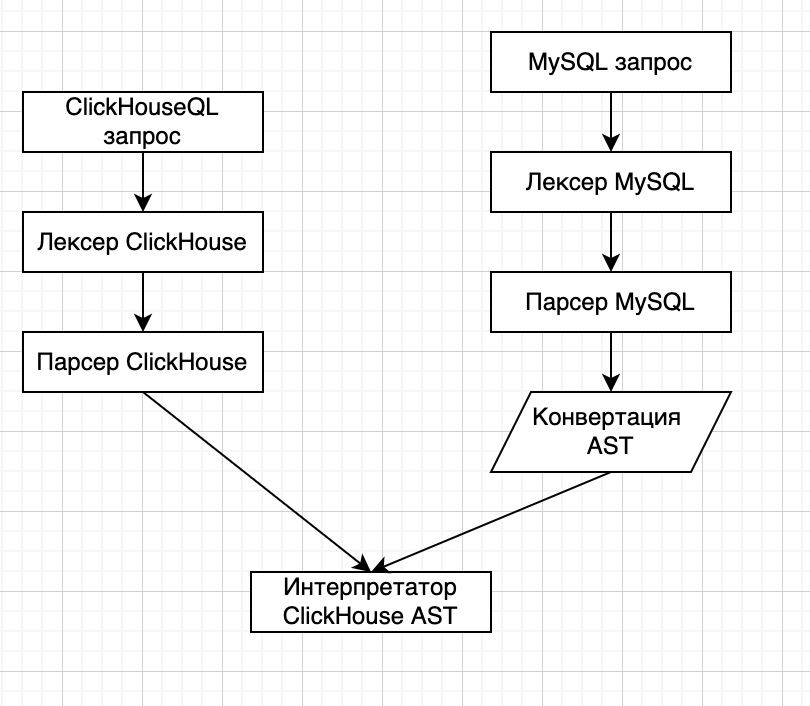
\includegraphics{images/general_conv_schema.jpg}
}
\caption{
\label{conv:general_pic} Общая схема конвертации MySQL запроса в диалект ClickHouse
}
\end{center}
\end{figure}

Ниже будут приведены фрагменты кода описывающие архитектуру конвертации MySQL AST в ClickHouse AST. Для большей лаконичности код упрощен и не содержит строк, не существенных для общего понимания архитектуры. Полноценные версии используемых классов и реализации методов могут быть найдены в ветке \textbf{antlr-mysql-parser} \textit{форка} репозитория ClickHouse, созданного в ходе выполнения данной работы \cite{my_branch}, а так же в соответствующем \textit{Merge Request} в основной репозиторий ClickHouse \cite{merge_request}.

Для выбора диалекта языка запросов в ClickHouse была добавлена опция \textit{sql\_dialect}, которая может принимать два значения: \textit{mysql} либо \textit{clickhouse} (по умолчанию). Изменить диалект запросов в ClickHouse можно двумя способами:

\begin{enumerate}
    \item Посредством указания опции в файле конфигурации:\\ \mintinline{xml}{<profiles>}\\\mintinline{xml}{<default><sql_dialect>mysql</sql_dialect></default>}\\ \mintinline{xml}{</profiles>}
    \item Посредством запроса вида \mintinline{sql}{SET sql_dialect='mysql'}. Этим же способом можно переключиться обратно на диалект ClickHouse, если до этого был выбран диалект MySQL, т. к. реализована поддержка запросов \mintinline{sql}{SET} на диалекте MySQL (см. Раздел \ref{part:queries})
\end{enumerate}

Для того чтобы успешно конвертировать ClickHouse AST в MySQL AST, необходимо извлечь нужную информацию из MySQL AST и придать ей структуру, соответствующую структуре, порождаемой парсером ClickHouse при разборе запроса \textit{семантически аналогичного} данному. Ниже изложен метод, позволяющий эффективно осуществлять подобное преобразование в общем случае.

Во фрагментах кода, приведенных ниже, за \mintinline{c++}{ MySQLPtr } обозначен умный указатель на MySQL AST, а за \mintinline{c++}{ CHPtr } - умный указатель на ClickHouse AST. Для поддержания общности будем называть \textit{исходным} тип AST, которое предстоит конвертировать (в данное работе - MySQL AST). Аналогично тип AST, которое должно быть результатом преобразования - \textit{целевым} (в данное работе - ClickHouse AST).

\subsection{Распознавание запроса} \label{conv:recognizer_}
Разбор запроса в ClickHouse устроен таким образом, что разным типам запросов соответствуют ClickHouse AST с корнями разных типов (в отличие от MySQL AST, корнем которого всегда является вершина с типом \textit{query}). Исходя из этого, было принято решение сделать \textbf{распознание запроса} первым шагом конвертации.

Распознавание основано на объектах, классы которых реализуют интерфейс \mintinline{c++}{ IRecognizer } (см. Листинг \ref{conv:IRecognizer_cpp}), содержащий в себе метод \mintinline{c++}{ IRecognizer::Recognize }. Этот метод принимает на вход вершину MySQL AST и определяет, содержится ли в ее поддереве \textbf{корень} дерева, соответствующего требуемому \textbf{типу запроса} (каждый наследник отвечает за специфический тип запроса). В случае успеха, метод возвращает вершину \textbf{дерева конвертации} (см. пункт \ref{conv_tree}), соответствующую корню нужного поддерева, в случае неудачи - \mintinline{c++}{ nullptr }.

\begin{code}
    \captionof{listing}{Архитектура распознавания запроса}
    \label{conv:IRecognizer_cpp}
    \begin{minted}[fontsize=\footnotesize, frame=single]{c++}
class IRecognizer
{
public:
    virtual ConvPtr Recognize(MySQLPtr node) const = 0;
    virtual ~IRecognizer() { }
};

class SelectQueryRecognizer : public IRecognizer
{
public:
    virtual ConvPtr Recognize(MySQLPtr node) const override;
};
    \end{minted}
\end{code}

Каждому типу запроса соответствует своей наследник класса \mintinline{c++}{ IRecognizer }. Для того, чтобы применить все правила к каждой вершине MySQL AST используется \mintinline{c++}{ GenericRecognizer } (см. Листинг \ref{conv:GenericRecognizer}), содержащий в себе список доступных правил (поле \mintinline{c++}{ rules }) и осуществляющий распознание посредством поиска в грубину с поочередным применением всех правил к каждой рассматриваемой вершине. Результатом обобщенного распознания является результат первого правила, вернувшего не \mintinline{c++}{ nullptr }. 

\begin{code}
    \captionof{listing}{Структура GenericRecognizer}
    \label{conv:GenericRecognizer}
    \begin{minted}[fontsize=\footnotesize, frame=single]{c++}
class GenericRecognizer : public IRecognizer
{
public:
    virtual ConvPtr Recognize(MySQLPtr node) const override;

private:
    std::vector<IRecognizerPtr> rules = {
            std::make_shared<SetQueryRecognizer>(),
            std::make_shared<SelectQueryRecognizer>(),
            std::make_shared<UseCommandRecognizer>(),
            std::make_shared<ShowQueryRecognizer>(),
            std::make_shared<DescribeCommandRecognizer>()
        };
}
    \end{minted}
\end{code}

На момент написания работы, в ClickHouse внедрена поддержка распознания следующих типов запросов:
\begin{itemize}
    \item Запросы типа \mintinline{sql}{SELECT}
    \item Запросы типа \mintinline{sql}{SHOW}
    \item Запросы типа \mintinline{sql}{USE}
    \item Запросы типа \mintinline{sql}{SET}
    \item Запросы типа \mintinline{sql}{DESCRIBE}
\end{itemize}

Запросы, не соответсвующее типам, указанным выше, не подлежат конвертации. При попытке исполнить неподдерживаемые запросы будет возвращена ошибка. Остальные запросы будут однозначно соответствовать поддерживаемым правилам, и будут конвертированы. Результатом конвертации может быть либо ClickHouse AST, семантически аналогичное исходному MySQL AST, либо ошибка указывающая на то, что данный запрос корректен, но несовместим с ClickHouse, несмотря на то, что его тип поддерживается.

В дальнейшем планируется расширять типы поддерживаемых запросов на диалекте MySQL, а так же уменьшать число ошибок конвертации поддерживаемых запросов путем добавления в ClickHouse недостающей функциональности. 

\subsection{Деревья конвертации} \label{conv_tree}
Выше было упомянуто, что каждое правило распознавания возвращает указатель на \textbf{дерево конвертации} в случае успеха. Дерево конвертации - предложенная в рамках данной работы концепция преобразования исходного AST в целевое путем создания древовидной сущности, структура которой зависит от данных, содержащихся в исходном AST и требуемой формы целевого AST одновременно. 

Принцип работы дерева конвертации состоит в двух последовательных шагах: извлечение деревом конвертации информации из исходного AST и порождение деревом конвертации целевого AST. Дерево конвертации конструируется от некоторой вершины исходного AST, которая в дальнейшем будет именоваться источником данных (\textit{source node}). В процессе извлечения данных дерево конвертации может исполнить 3 типа действий:

\begin{enumerate}
    \item Сохранить в свои поля любые данные, содержащиеся в поддереве собственного источника данных, в подходящем формате
    \item Создать дочернее дерево конвертации, взяв за источник данных вершину, лежащую в поддереве собственного источника данных, после чего инициировать у него процесс извлечения данных, а затем записать его (но не данные им извлеченные) в свое поле. 
    \item Вернуть ошибку, если в источнике данных присутствует информация, которую дерево конвертации не ожидает встретить или не может обработать
\end{enumerate}

На втором шаге (порождение целевого AST), дерево конвертации возвращает \textbf{ровно одну} вершину целевого AST (возможно, с потомками). Для этого дерево конвертации может исполнить 4 типа действий:

\begin{enumerate}
    \item Создать вершину целевого AST используя собственные поля, соответствующие извлеченным данным (полученным путем действия типа 1 на шаге 1)
    \item Инициировать процесс порождения вершины целевого AST у одной из собственных \textbf{дочерних} вершин конвертации (полученных путем действия типа 2 на шаге 1)
    \item Образовать связь между любыми двумя вершинами целевого AST, полученными действиями 1 и 2
    \item Назначить одну из полученных вершин результатом (после создания необходимых связей) и завершить работу
\end{enumerate}

Структура дерева конвертации и его действия должны удовлетворять следующим требованиям
\begin{enumerate}
    \item Если процесс извлечения данных завершился ошибкой, порождение целевого AST не инициируется
    \item В процессе порождения целевого AST запрещается обращаться к исходному AST, а так же изменять структуру и поля дерева конвертации (включая дочерние деревья конвертации)
    \item Дерево конвертации не должно извлекать данные из поддеревьев, соответствующих источникам данных его дочерних деревьев конвертации
\end{enumerate}

Предложенный метод обладает следующими важными положительными свойствами:
\begin{enumerate}
    \item Процесс порождения целевого дерева не зависит от структуры исходного дерева и деталей алгоритма извлечения данных (по построению алгоритма)
    \item Процесс порождения целевого дерева не может завершиться ошибкой и его результат всегда корректен (причиной ошибки может быть только неподдерживаемая структура исходного дерева, что определяется на шаге 1)
    \item После извлечения данных, дерево конвертации может породить произвольное количество идентичных целевых деревьев (следует из того, что в процессе порождения не меняется ни исходное AST, ни дерево конвертации)
\end{enumerate}

\subsection{Применение деревьев конвертации в ClickHouse}
Предложенная концепция дерева конвертации была реализована в ClickHouse с целью конвертировать MySQL AST в ClickHouse AST. Вершины дерева реализуют интерфейс \mintinline{c++}{ IConversionTree }, включающий в себя методы \mintinline{c++}{ IConversionTree::setup } (реализует извлечение данных из исходного AST) и \mintinline{c++}{ IConversionTree::convert } (реализует порождение целевого AST), а так же поле \mintinline{c++}{ IConversionTree::_source } - источник данных (см. Листинг \ref{conv:IConversionTree_cpp}).

\begin{code}
    \captionof{listing}{Интерфейс дерева конвертации}
    \label{conv:IConversionTree_cpp}
    \begin{minted}[fontsize=\footnotesize, frame=single]{c++}
class IConversionTree
{
public:
    IConversionTree(MySQLPtr source, const String & rule_name = "");
    virtual bool setup(String & error) = 0;
    virtual void convert(CHPtr & ch_tree) const = 0;
    virtual ~IConversionTree() { }

protected:
    MySQLPtr getSourceNode() const { return _source; }

private:
    MySQLPtr _source; // source node
};

using ConvPtr = std::shared_ptr<IConversionTree>;
    \end{minted}
\end{code}

На момент написания работы были реализованы следующие типы вершин конвертации:
\begin{enumerate}
    \item Деревья конвертации выражений \begin{enumerate}
        \item ExprGenericLiteralCT - конвертирует литералы (число, строка, TRUE, FALSE, NULL, и т. д.)
        \item ExprIdentifierCT - конвертирует идентификаторы (имена столбцов, алисов и т. д.)
        \item ExprVariableCT - конвертирует переменные
        \item ExprSumCT - конвертирует агрегатные функции
        \item ExprSimpleCT - конвертирует выражения с унарным минусом и вызовы функций
        \item ExprBitCT - конвертирует арифметические операции
        \item ExprBoolStatementCT - конвертирует выражения, которые могут быть простыми логическими высказываниями
        \item ExpressionCT - конвертирует выражения, которые могут быть сложными логическими высказываниями
    \end{enumerate}
    \item Деревья конвертации запроса \mintinline{sql}{ SELECT } \begin{enumerate}
        \item SelectItemsListCT - конвертирует список выбираемых элементов
        \item SelectOrderByCT - конвертирует клаузу \mintinline{sql}{ ORDER BY } 
        \item SelectLimitOffsetCT - конвертирует смещение в выражении \mintinline{sql}{ LIMIT } 
        \item SelectLimitLengthCT - конвертирует размер в выражении \mintinline{sql}{ LIMIT } 
        \item SelectTableCT - конвертирует идентификатор таблицы
        \item SelectFromCT - конвертирует клаузу \mintinline{sql}{ FROM } 
        \item SelectGroupByCT - конвертирует клаузу \mintinline{sql}{ GROUP BY} 
        \item SelectQueryExprCT - конвертирует запрос \mintinline{sql}{ SELECT }
        \item SelectQueryCT - вспомогательное дерево, нужное для совместимости с ClickHouse AST
    \end{enumerate}
    \item Деревья конвертации запроса \mintinline{sql}{ SHOW } \begin{enumerate}
        \item ShowColumnsCT - конвертирует запрос вида \mintinline{sql}{ SHOW COLUMNS } 
        \item ShowTablesCT - конвертирует запрос вида \mintinline{sql}{ SHOW TABLES; } 
        \item ShowQueryCT - конвертирует запросы \mintinline{sql}{ SHOW } в общем виде 
    \end{enumerate}
    \item Прочие деревья конвертации \begin{enumerate}
        \item SetQueryCT - конвертирует запросы \mintinline{sql}{ SET } 
        \item UseCommandCT - конвертирует запрос \mintinline{sql}{ USE databasee; } 
        \item DescribeCommandCT - конвертирует запрос \mintinline{sql}{ DESCRIBE }
    \end{enumerate}
\end{enumerate}

Точка входа, запускающая процесс распознания запроса, с последующим созданием и использованием дерева конвертации выглядит следующим образом (см. Листинг \ref{conv:EntryPoint}):

\begin{code}
    \captionof{listing}{Точка входа в процесс конвертации}
    \label{conv:EntryPoint}
    \begin{minted}[fontsize=\footnotesize, frame=single]{c++}
bool Converter::toClickHouseAST(const String & query, 
                CHPtr & ch_tree, String & error) const
{
    MySQLPtr root = nullptr;
    MySQLTree::FromQuery(query, root, internal_error);

    // invalid MySQL query error handling

    GenericRecognizer recognizer;
    
    auto result = recognizer.Recognize(root);
    result->setup(internal_error);

    // failed conversion error handling

    result->convert(ch_tree);

    return true;
}
    \end{minted}
\end{code}

\begin{figure}[ht]
\begin{center}
\scalebox{0.25}{
    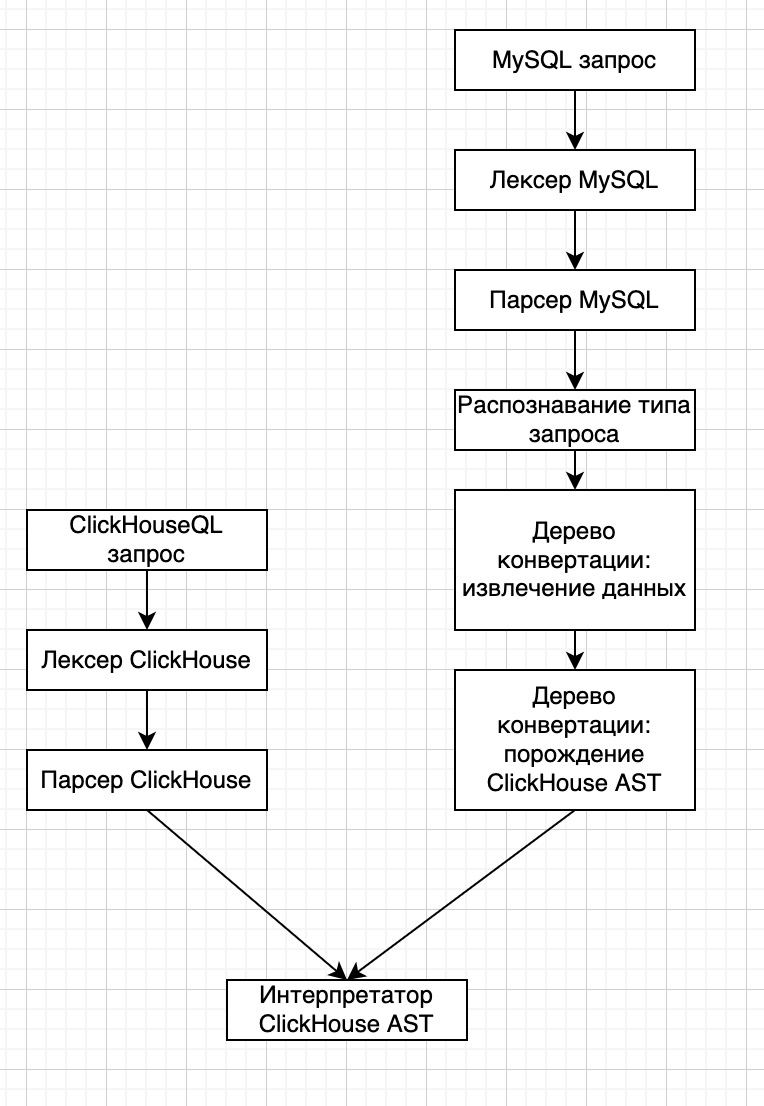
\includegraphics{images/spec_conv_schema.jpg}
}
\caption{
\label{conv:spec_pic} Схема конвертации MySQL AST в ClickHouse AST
}
\end{center}
\end{figure}


С учетом описанного выше, схему архитектуры процесса конвертации запроса на диалекте MySQL в ClickHouse, изложенную в начале главы (см. Рис. \ref{conv:general_pic}), можно дополнить до следующего вида (см. Рис. \ref{conv:spec_pic}):

\subsection{Множество поддерживаемых запросов} \label{part:queries}
Алгоритм преобразования MySQL AST в ClickHouse AST, использующий метод деревьев конвертации позволил поддержать следующее подмножество корректных запросов на диалекте MySQL:
\begin{itemize}
    \item Запрос \mintinline{sql}{ USE databasee; }
    \item Запрос \mintinline{sql}{ DESCRIBE table; }
    \item Запрос вида \mintinline{sql}{ SET key1=val1, key2=val2, ... }, где key - переменная, а val - литерал
    \item Запросы вида \mintinline{sql}{ SHOW TABLES } и \mintinline{sql}{ SHOW COLUMNS FROM }
    \item Запросы \mintinline{sql}{ SELECT }:
    \begin{itemize}
        \item Не содержащие \mintinline{sql}{ JOIN } и \mintinline{sql}{ UNION }
        \item Поддерживающие выражения в списке выбираемых элементов
        \item Поддерживающие \mintinline{sql}{ WHERE }, \mintinline{sql}{ ORDER BY }, \mintinline{sql}{ GROUP BY }, \mintinline{sql}{ HAVING } и \mintinline{sql}{ LIMIT }
        \item Поддерживающие агрегатные функции 
        \begin{itemize}
            \item \mintinline{sql}{ sum }
            \item \mintinline{sql}{ count }
            \item \mintinline{sql}{ min }
            \item \mintinline{sql}{ max }
            \item \mintinline{sql}{ avg }
            \item \mintinline{sql}{ stddev_pop}
            \item \mintinline{sql}{ stddev_samp }
            \item \mintinline{sql}{ var_pop }
            \item \mintinline{sql}{ var_samp }
        \end{itemize}
        \item Поддерживающие подзапросы вида \\ \mintinline{sql}{ SELECT ... FROM (SELECT ...) ...; }
    \end{itemize}
\end{itemize}

Поддерживаемый синтаксис не является исчерпывающим, однако предложенный метод конвертации позволяет легко итеративно расширять подмножество поддерживаемых запросов.


\section{Тестирование} \label{chap:testing}
Для того, чтобы проверить корректность предложенного в данной работе метода конвертации абстрактных синтаксических деревьев, в ClickHouse были добавлены автоматизированные тесты, провереряюще: корректность работы парсера MySQL (юнит-тесты), корректность конвертации запросов на диалекте MySQL (функциональные тесты)

\subsection{Юнит-тесты}
В исходном репозитории выбранного MySQL парсера содержатся тесты, проверяющие его корректность. Их основой служит файл \textbf{statements.txt} с запросами, которые парсер MySQL должен преобразовать в дерево разбора без ошибок (см. Главу \ref{chap:mysql}).

Используя этот файл из исходного репозитория мною был написаны два юнит-теста, проверяющие корректность MySQL парсера встроенного в кодовую базу ClickHouse. ClickHouse использует фреймворк \textit{GoogleTest} в качестве инструмента для юнит-тестирования.

Первый юнит тест содержит простые запросы, выбранные из общего множества тестовых запросов, и проверяет корректность построенного по дереву разбора MySQL AST.

Второй юнит тест содержит все множество тестовых запросов и проверяет, что все запросы из этого множества обрабатываются без ошибок (корректность итогового MySQL AST не проверяется). Поскольку множество тестовых запросов включает в себя порядка 1000 запросов, было принято решение написать \textit{скрипт}, генерирующий исходный код теста на основе файла \textbf{statements.txt}, который был скопирован в директорию с юнит-тестами из исходного репозитория парсера

\subsection{Функциональные тесты}
Помимо тестов, проверяющих корректность работы парсера MySQL самого по себе, были написаны тесты, проверяющие корректность интерпретации запросов на диалекте MySQL в ClickHouse (функциональные тесты). ClickHouse использует собственный фреймворк, позволяющий осущеcтвлять функциональное тестирование. В простом случае (исключая специфичные тесты, которые не затрагивают данную работу) тест состоит из файла с расширением \textit{.sql}, описывающего последовательность запросов, и файла с расширением \textit{.ref} (refference file), содержащего \textit{ожидаемый ответ} ClickHouse на заданную последовательность запросов

Для проверки корректности метода конвертации в набор функциональных тестов ClickHouse были добавлены 2 теста:
\begin{enumerate}
    \item Тест, проверяющий корректность работы запросов \mintinline{sql}{ SELECT } на диалекте MySQL, не использующих таблицы. Тест проверяет корректность обработки выражений, фильтрацию комментариев и прочие базовые инварианты
    \item Тест, проверящий корректность поддерживаемых запросов на диалекте MySQL, работающих с таблицами. Проверяются запросы вида \mintinline{sql}{ USE database; }, \mintinline{sql}{ SHOW }, \mintinline{sql}{ DESCRIBE }, \mintinline{sql}{ SET }, а так же корректность работы операторов \mintinline{sql}{ LIMIT }, \mintinline{sql}{ WHERE }, \mintinline{sql}{ ORDER BY }, \mintinline{sql}{ GROUP BY }, \mintinline{sql}{ HAVING }, агрегатные функции и подзапросы.
\end{enumerate}

Тесты предполагают, что конфигурационный файл ClickHouse \textbf{не} содержит опции, включающей использование диалекта MySQL по умолчанию. Вместо этого в начале каждого теста, всем группам запросов на диалекте MySQL предшествует команда \mintinline{sql}{ SET sql_dialect = 'mysql';} (см. Главу \ref{chap:conversion}), последним запросом каждого теста является команда \mintinline{sql}{ SET sql_dialect='clickhouse'; }, возвращающая ClickHouse к собственному диалекту (для корректной работы с другими тестами)

\pagebreak


\section{Результаты} \label{chap:results}
Непосредственным результатом дипломной разботы является Pull Request в основной репозиторий ClickHouse, содержащий код, интегрирующий парсер MySQL в ClickHouse и позволяющий ClickHouse работать в режиме диалекта MySQL, распознавая некоторое подмножество запросов на этом диалекте

\subsection{Метод конвертации}
В рамках данной работы не удалось поддержать в ClickHouse синтаксис MySQL целиком, более того, большинство типов запросов не распознаются на начальном этапе с последующим возвратом ошибки (см. Раздел \ref{conv:recognizer_}).

Несмотря на это, в работе предложена концепция \textit{деревьев конвертации}, которая была реализована в обозначенном выше Pull Request в качестве метода конвертации AST. Ее использование позволит постепенно увеличивать совместимсть ClickHouse с диалектом MySQL вплоть до полной совместимости (возможно, ограниченной факторами, не относящимися непосредственно к языку запросов). 

\subsection{Совместимость с Google Data Studio} \label{res:google}
Корректность представленного в данной работе решения может быть проверена не только синтетическими авто-тестами, которые можно найти в Pull Request. Совместимость ClickHouse с диалектом MySQL была проверена путем интеграции ClickHouse c Google Data Studio (веб-сервис, позволяющий визуализировать данные под управлением СУБД)

На удаленном хосте, доступном из внешней сети, была размещена программа \textit{clickhouse}, скомпилированная из ветки, содержащей изменения, описанные в данной работе (описанные в Pull Request, упомянутом выше). Был запущен сервер ClickHouse с конфигурационным файлом, предписывающим ClickHouse использовать диалект MySQL по умолчанию для всех подключений (см. Раздел \ref{conv:general_}). С использованием собственного диалекта, в ClickHouse были созданы тестовые таблицы вместе с содержимым

После этого Google Data Studio была подключена к серверу ClickHouse посредством \enquote{коннектора MySQL}. Затем была создана страница, включающие в себя элементы визуализации, которые предоставляет Google Data Studio (TODO: ССЫЛКА КОТОРАЯ В ТЕЛЕГЕ). ClickHouse в режиме работы с MySQL диалектом успешно обработал запросы, полученные от Google Data Studio, что говорит корректности реализованного решения

В ходе интеграции ClickHouse в режиме работы с диалектом MySQL обнаружилось, что Google Data Studio не может успешно подключться к серверу через графический интрфейс, хотя подключение через запрос происходит успешно. Применяя \textit{reverse engineering}, было установлено, что проблема заключается в том, что Google Data Studio не может успешно обработать ответ на запрос вида \mintinline{sql}{ DECRIBE table }, хотя ClickHouse его обрабатывает без ошибок и возвращает корректный результат. Прична такого поведения - несоответсвие \textit{формата вывода} ответа на данный запрос, что выходит за рамки данной работы. 

\subsection{Дальнейшее направление работы}
Данная работа предлагает метод конвертации AST и демонстрирует его работу на примере реализации поддержки диалекта MySQL в ClickHouse, что делает ее завершенной и самодостаточной

Однако, за рамками дипломной работы остается множество направлений для дальнейшей разработки, которые станут частью работы по внедрению полученных результатов в основной репозиторий ClickHouse:
\begin{enumerate}
    \item Поддержать новые типы запросов (\mintinline{sql}{ UPDATE }, \mintinline{sql}{ INSERT }, \mintinline{sql}{ DELETE } и т. д.)
    \item Улучшить совместимость ClickHouse с уже поддерживаемым типами запросов (например добавить поддержку \mintinline{sql}{ JOIN } и \mintinline{sql}{ UNION } в запросы \mintinline{sql}{ SELECT }
    \item Поддержать альтернативные форматы вывода в зависимости от выбранного диалекта SQL (с целью решить проблему, обозначенную в конце Раздела \ref{res:google})
    \item Расширить список сторонних инструментов, совместимых с ClickHouse, работающем в режиме поддержки диалекта MySQL (phpMyAdmin, adminer, Sequel Ace и т. д.)
\end{enumerate}

\pagebreak


% Библиография в cpsconf стиле
% Аргумент {1} ниже включает переопределенный стиль с выравниванием слева
\begin{thebibliography}{1}
\bibitem{voc} Griffin D.W., Lim J.S. \flqq Multiband excitation vocoder\frqq. IEEE ASSP-36 (8), 1988, pp. 1223-1235.
\bibitem{vo2} Griffin D.W., Lim J.S. \flqq Multiband excitation vocoder\frqq. IEEE ASSP-36 (8), 1988, pp. 1223-1235.
\end{thebibliography}


\end{document}
